\section{Evaluation and benchmarking}

In order to develop robust system, we have decided to focus on intensive testing and evaluation. 
Therefore, we tried to find possibilities how to built a test arena and equipped it by real objects.
However, this is impossible for us due to strongly limited budget and no space. 
Although, we came up with a better idea - we have decided to use flat of one of us, see Fig.~\ref{fig:kitchen}.
Hence, our robot is deployed permanently in this flat now and we record datasets during regular testing which we plan publish later. 

We have found such environment really close to the arena with all tricky situations such as narrow corridors, door steps, a large mirror, etc. 
Therefore, we are able to test our algorithms in a realistic environment and improve their robustness.
We created a video from our testing, which can be found on our websites~\cite{barc_web}. More detailed description of our evaluation will be publish there before the competition in November.

\begin{figure}[ht!b]
\centering
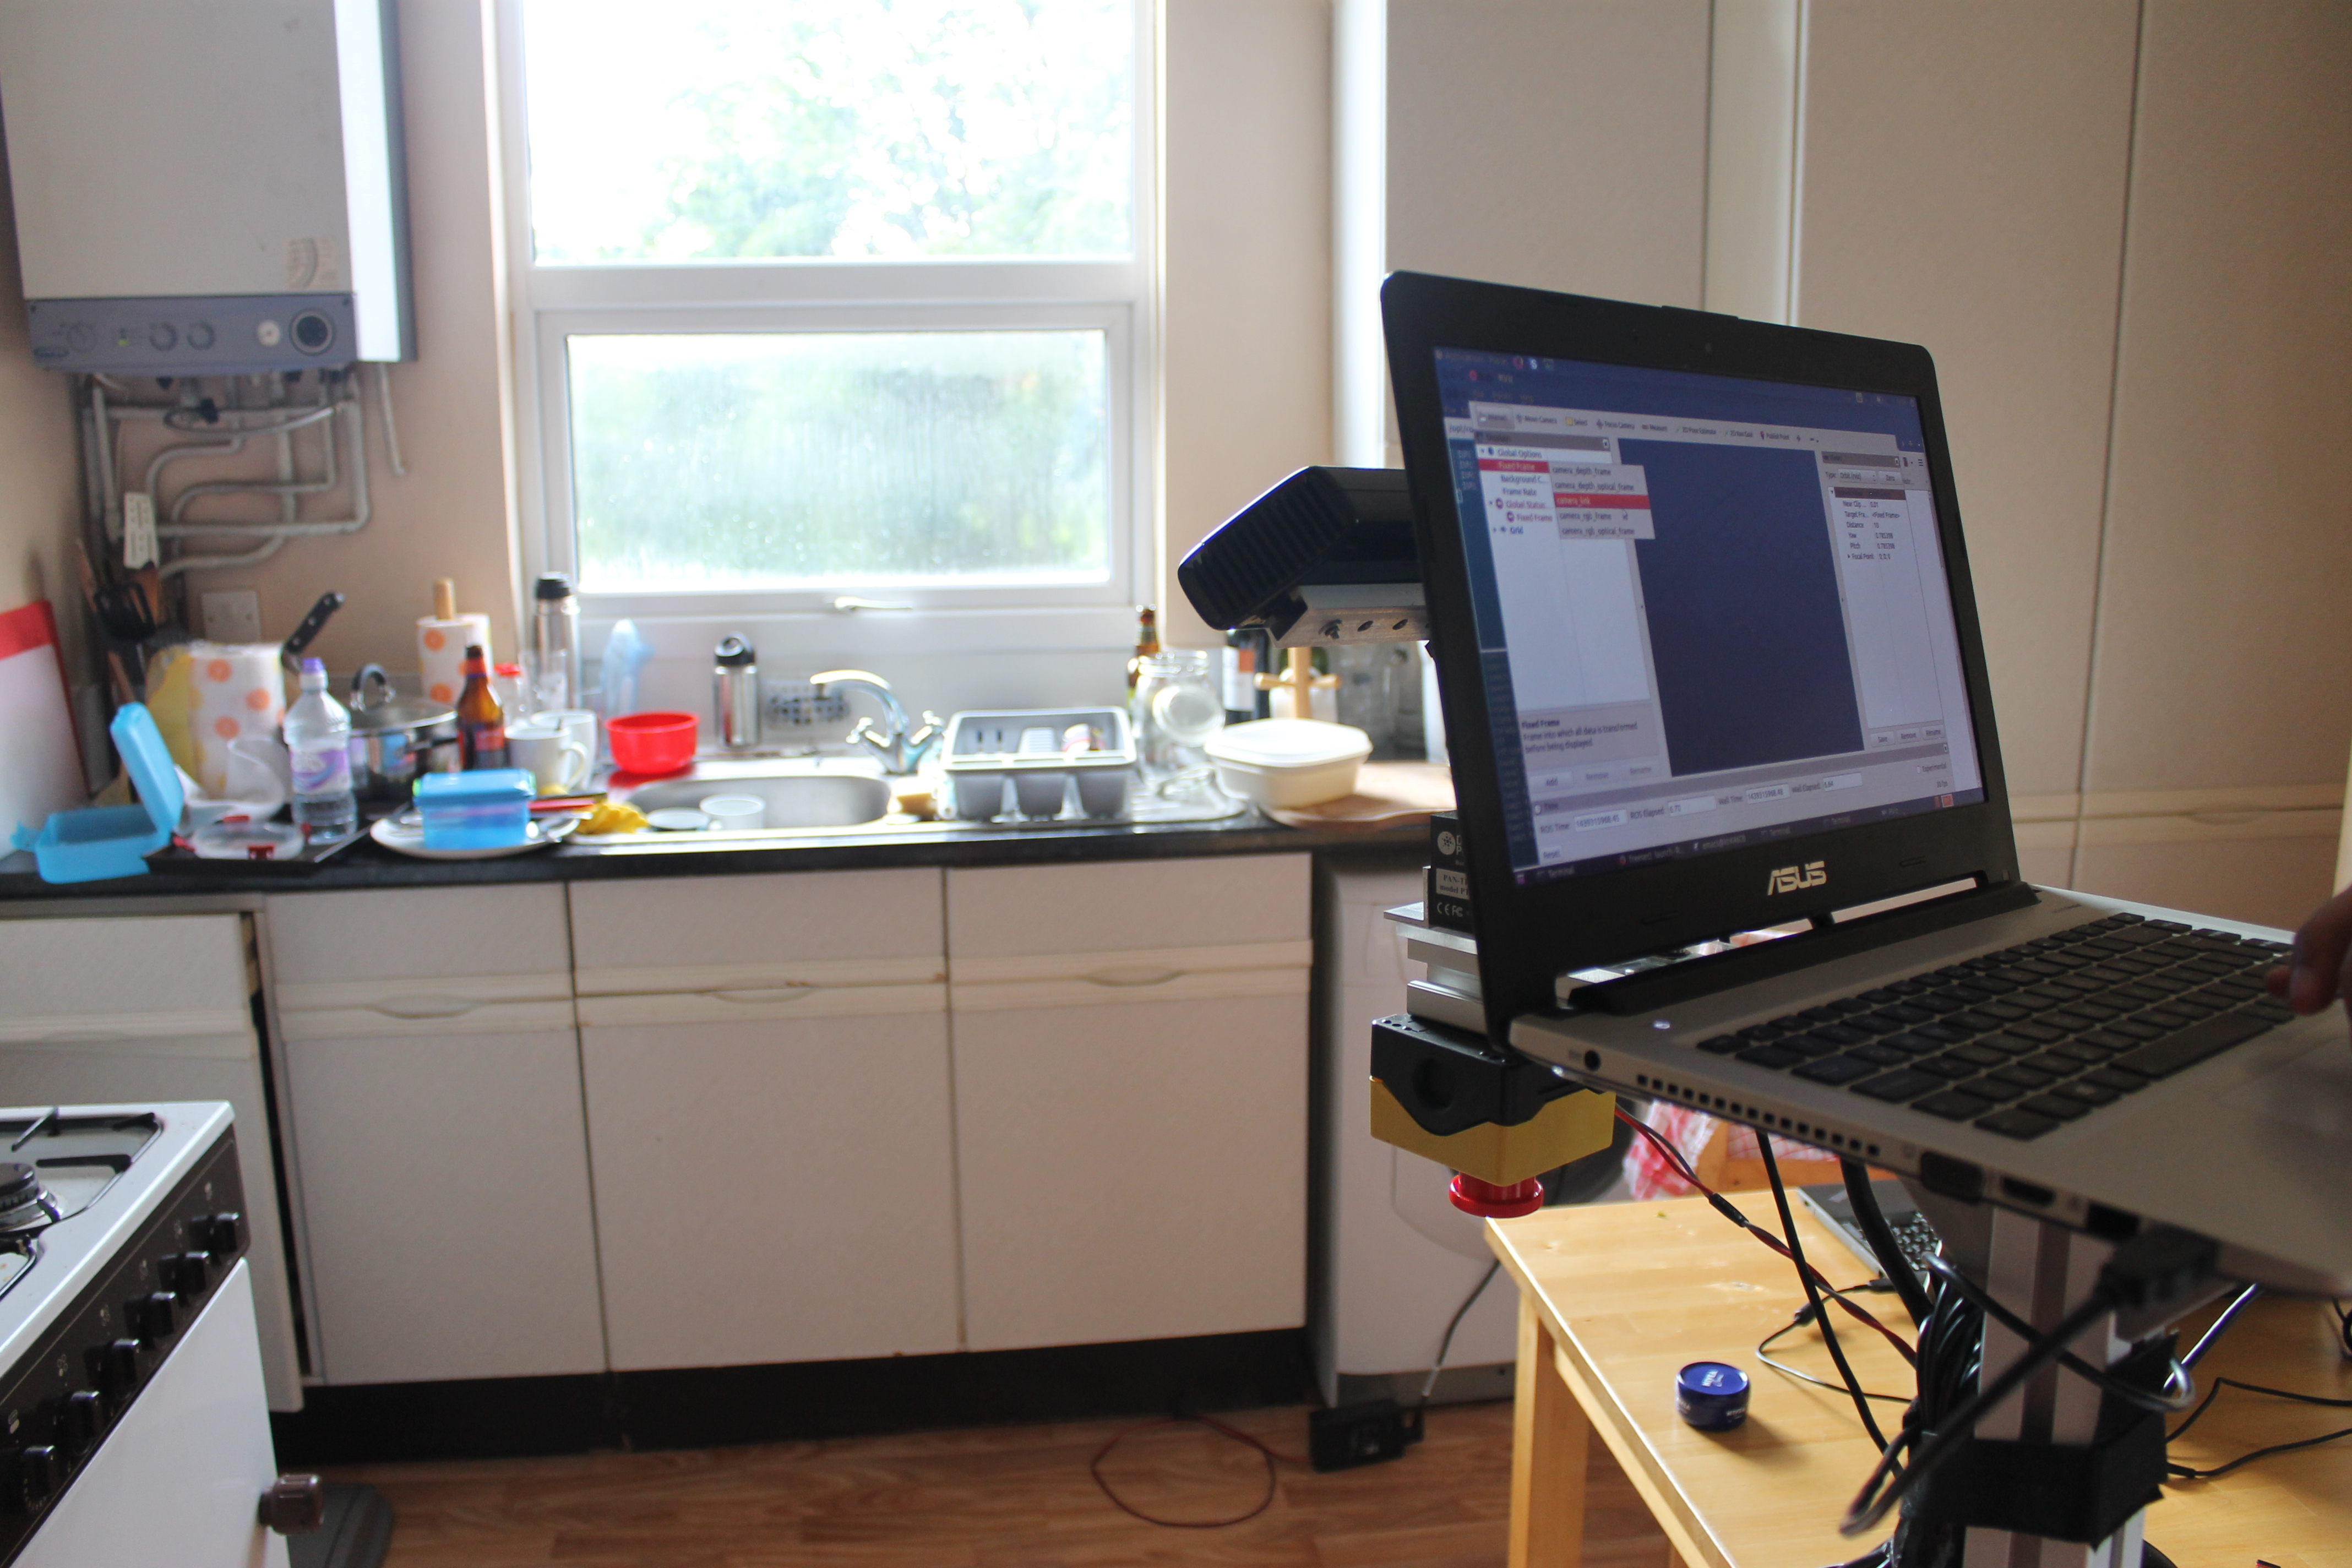
\includegraphics[width=3.in]{kitchen.JPG}
\caption{Long-term deployment of Dora in a flat}
\label{fig:kitchen}
\end{figure}  